\subsubsection{Kopfbeleuchtung}
\label{subsubsec:led}

Die \gls{led}-Reihen an den beiden Außenseiten des Kopfes sind, wie in Kapitel \ref{sec:roboterarchitektur-und-systemkomponenten}
beschrieben, am Jetson Nano des Kopfes angeschlossen.
Prüft man dort die Funktionen, die über den Autostart gesteuert werden, so fallen zwei Ordner auf -- \texttt{faceLightServer/}
und \texttt{faceLightMqtt/}.
Leider sind die Funktionalitäten beider Skripte als Binärdateien abgelegt und somit nicht ohne weiteres auslesbar.
Auch die Dokumentation des Herstellers weist keinerlei Informationen zu den \gls{led}-Reihen auf.
Der Name des zweiten Ordners weist jedoch auf eine mögliche Funktionalität der Steuerung über MQTT hin.
Um dies zu bestätigen, lässt sich ein MQTT-Explorer verwenden.
Dieser registriert sich als Client beim MQTT-Broker und schreibt alle Nachrichten und veröffentlichten Topics mit.
Mehr zum Thema MQTT gibt es auf der offiziellen Dokumentation des Standards\footnote{https://mqtt.org/}, Beispiele zur Nutzung
des Standards am Roboter in Kapitel \ref{sec:funktionserweiterungen-und-integration}.

Zur Nutzung des MQTT Explorers wird die \gls{ip}-Adresse des Brokers und der Port, auf dem dieser veröffentlicht wird, benötigt.
Für die Adresse kommen nur die \glspl{ip} \texttt{192.168.123.13}, \texttt{...14}, \texttt{...15} und \texttt{...161}
infrage.
Es kann mit der Bibliothek \emph{Nmap} geprüft werden, ob der MQTT-Standardport \texttt{1883} auf einer der registrierten \glspl{ip}
im Netz \texttt{192.168.123.0/24} geöffnet ist.

\begin{lstlisting}
nmap -sS -O -p1883 192.168.123.0/24
\end{lstlisting}

\noindent Die Ausgabe zeigt, dass die beiden \glspl{ip}
\texttt{192\allowbreak .168\allowbreak .123\allowbreak .15} und \texttt{192\allowbreak .168\allowbreak .123\allowbreak .161} den MQTT Port offen haben.
Über den MQTT Explorer wird zunächst der NVIDIA Jetson Xavier NX als Broker getestet.
Die Verbindung funktioniert, jedoch werden weder verfügbare Topics noch Messages ausgegeben.
Ein Test auf dem Raspberry Pi mit der \gls{ip} \texttt{192.168.123.161} zeigt die Ausgabe wie in Abbildung \ref{fig:mqtt-explorer}
dargestellt.

\begin{figure}[h]
    \frame{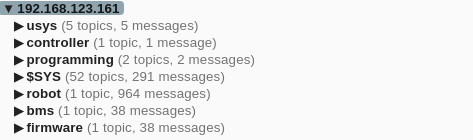
\includegraphics[width=\linewidth]{img/analyse/mqtt-explorer-no-facelight}}
    \caption{Ausgabe eines MQTT Explorers in Verbindung mit dem Raspberry Pi als Broker}\label{fig:mqtt-explorer}
\end{figure}

In den angezeigten Topics sind aktuell noch keine Informationen zu den \glspl{led} zu erkennen.
Dies kann daran liegen, dass das zu dem Topic noch keine Nachrichten versendet wurden, was eine plausible Schlussfolgerung
ist, da die Kopflichter des \gls{go1} standardmäßig ausgeschalten sind.
Ändert man dies nun durch die in der mobilen Anwendung gegebenen Funktion unter dem Menüpunkt \texttt{Preferences}, so
sieht man auch das Topic \texttt{face\_light/color} im MQTT-Explorer, wie in Abbildung \ref{fig:app-mqtt-facelight} dargestellt.

\begin{figure}[h]
    \frame{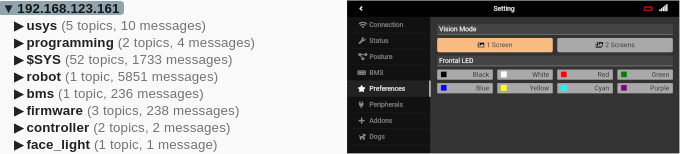
\includegraphics[width=\linewidth]{img/analyse/app-mqtt-facelight}}
    \caption{MQTT Explorer mit Topic \texttt{face\_light/color} (links) und App-Funktion (rechts)}\label{fig:app-mqtt-facelight}
\end{figure}

Die Message Payload kann beispielsweise über das Commandline-Tool \emph{Mosquitto-Client} ausgegeben werden.
Hierfür muss folgender Befehl genutzt werden, um die binäre Payload lesbar auszugeben.
Der genutzte Rechner muss sich hierfür im Netzwerk des \gls{go1} befinden.

\begin{lstlisting}
mosquitto_sub -h 192.168.123.161 -t face_light/color -F %x
ff0000
00ff00
0000ff
\end{lstlisting}

\noindent Die drei Werte in den letzten der Zeilen der Ausgabe sind formatierte Message-Payloads des Topics \texttt{face\_light/color}
und wurden ausgegeben, als in der mobilen Anwendung die drei Farben \emph{Rot}, \emph{Grün} und \emph{Blau} in eben dieser
Reihenfolge eingestellt wurden.
Somit ist herleitbar, dass die \glspl{led} des Roboters über den \emph{RGB}-Farbraum konfigurierbar sind.
Die Mischung aus Rot, Grün und Blau kann hier pro Farbe mit einem Wert von \num{0} - \num{255} eingestellt werden.

Über den Befehl \texttt{mosquitto\_pub} kann nun auch die Farbe des Roboters geändert werden.
Hierfür muss nur das Versenden der Message-Payload in binärer Form beachtet werden.
Folgender Befehl stellt das Kopflicht des \gls{go1} auf Rot um.

\begin{lstlisting}
echo -ne "\xFF\x00\x00" | mosquitto_pub -h 192.168.123.161 -t face_light/color -s
\end{lstlisting}

\noindent Es ist ebenfalls denkbar die \glspl{led} des Roboters direkt über die \texttt{CP210x UART Bridge} zu steuern, die in Kapitel
\ref{par:nano-kopf} erwähnt wurde.
Dies wurde im Rahmen dieser Arbeit jedoch nicht umgesetzt und kann in Zukunft noch dokumentiert werden.
